\documentclass[conference]{IEEEtran}
\IEEEoverridecommandlockouts

\usepackage{cite}
\usepackage{amsmath,amssymb,amsfonts}
\usepackage{graphicx}
\usepackage{textcomp}
\usepackage{xcolor}
\usepackage{subcaption}
\usepackage{float} 
\usepackage{verbatim}
\usepackage{subfig}
\usepackage{graphicx} % already needed for resizebox

\def\BibTeX{{\rm B\kern-.05em{\sc i\kern-.025em b}\kern-.08em
    T\kern-.1667em\lower.7ex\hbox{E}\kern-.125emX}}

\begin{document}

\title{Analyzing Sales Performance and Profitability Across Regions Using Interactive Tableau Dashboards
\\
}

\author{
\IEEEauthorblockN{1\textsuperscript{st} Haji Qasim}
\IEEEauthorblockA{
\textit{Department of AI \& Data Science} \\
\textit{National University of Computer and} \\
\textit{Emerging Sciences} \\
Islamabad, Pakistan \\
i248011@isb.nu.edu.pk}
\and 
\IEEEauthorblockN{2\textsuperscript{nd}Rahmat Ullah}
\IEEEauthorblockA{
\textit{Department of Software Engineering} \\
\textit{National University of Computer and} \\
\textit{Emerging Sciences} \\
Islamabad, Pakistan \\
i247804@isb.nu.edu.pk}
\and 
\IEEEauthorblockN{3\textsuperscript{rd}Arif Hussain}
\IEEEauthorblockA{
\textit{Department of AI \& Data Science} \\
\textit{National University of Computer and} \\
\textit{Emerging Sciences} \\
Islamabad, Pakistan \\
i248047@isb.nu.edu.pk}

}

\maketitle


\begin{abstract}
The growing amount of transactional data in multinationally operated retail businesses poses a challenge in deriving meaningful insights to inform decisions. The interactive visual analysis of the dataset of the Global Superstore is proposed in this research to analyse the sales performance and profitability in the various regions. The methodology implies preprocessing the data in Python, including data cleaning, type conversion, and feature creation, and the creation of a Tableau dashboard that includes the key indicators, such as total sales, total profit, number of orders and average discount. The dashboard has times based analysis, category level comparison, regional performance view and a scatter plot to analyse the relationship between discount and profit. The interactive capabilities enable users to filter and highlight data in many views to support step by step exploration of summary to detail. The analysis shows that there is a huge issue in Furniture category and the high sales are connected with negative profit. It also shows a clear negative relationship between the level of discounts and profit margin, that is, increase in the level of discounts has negative effect on profitability. These results demonstrate that pricing and category management need to be carefully adjusted. The study also shows that interactive dashboards can help in getting a clear understanding of the business data and help the decision makers to identify performance issues and work on improving operational strategies.
\end{abstract}

\begin{IEEEkeywords}
Data Visualization, Business Intelligence, Tableau Dashboard, Sales Analysis, Profitability Analysis, Interactive Dashboards, Visual Analytics, Retail Analytics, Data Preprocessing, Exploratory Data Analysis
\end{IEEEkeywords}


\section{Introduction}
The extensive proliferation of data in contemporary retail and enterprise settings has greatly heightened the significance of Business Intelligence (BI) and data visualization tools in making effective decisions. Organizations have found themselves in huge amounts of transactional data in various regions, customer segments, and product categories, and the traditional analysis methods are inadequate to extract actionable insights. The interactive visualization systems have found their way as a compelling solution, giving users the opportunity to explore complex data sets through intuitive visual interfaces and supporting analytical reasoning through techniques such as filtering, highlighting, and drill down exploration \cite{few2006information, shneiderman1996eyes}.

Even though these developments have been made, multinational organizations continue to experience significant challenges in checking and analyzing sales performance and profitability in the various global markets. The differences in the regional demand, customer behavior, discounts strategy, and shipping methods add complexity in determining key performance drivers. In particular, the correlation of sales growth, profit margins and operational issues (i.e. discounting policies and shipping priorities) is not a trivial matter. These issues have led to the need to have a single analytical framework, which converts different performance metrics into a coherent and interactive perspective.

Before visualization, the data set of this study, the Global Superstore dataset was thoroughly preprocessed using Python as provided in the supplemental notebook. The preprocessing pipeline involved verification of data integrity, non null values of all the attributes, conversion of date fields into the appropriate datetime format and derivation of other analytical features like year, month, profit ratio, and profit category. In addition, the redundant attributes were deleted and numerical stability was established through the extreme and missing values, to prepare the dataset to be consistently and accurately visualized.

To respond to the challenges identified, in this study, the interactive Tableau based dashboard, which is built on consolidating key performance indicators (KPIs), such as total sales, total profit, order number, and average discount, into a single analytical platform is proposed. The dashboard incorporates various visualization methods so as to give an integrated picture of the business performance. These involve the time series analysis of sales trends between customer segments, comparative analysis of sales and profit between product categories, analysis of regional and market level distribution of performance and analysis of the relationship between discount levels and profit margins where higher discounts are observed negatively affecting profitability.

The main characteristic of the proposed system is that it is interactive, which is ensured by cross chart linking and dashboard actions. Users can interactively investigate the relationships in the data by selecting elements in one visualization and seeing the corresponding changes in others, such as highlighting category specific patterns in scatter plots or filtering KPI metrics based on temporal selections. This interactive feature helps to support a top down exploratory analysis model, which allows the user to smoothly transition between the aggregated insights and the detailed observations.

The rest of this paper is structured in the following way. Part II is a literature review of related work in the field of business intelligence and data visualization. Section III describes the dataset and preprocessing methodology. Section IV describes the design and implementation of interactive dashboard. Section V argues the findings and conclusions based on the analysis of the visual analysis. Lastly, Section VI wraps up the paper and describes the possible future work.
\section{Literature Review}

Business Intelligence (BI) has evolved to be much more than its counterparts in business reporting systems, which are mostly static reporting platforms designed to deliver reports, rather than facilitate dynamic data exploration and decision support. The early versions of BI systems were mainly centered around pre-defined reports and dashboards that only allowed users to view fixed views of aggregated information. Nevertheless, the advent of interactive visualization tools has changed this paradigm as it enables users to manipulate, filter and explore data in real time. Non-technical users have been enabled to perform complex analytical tasks through intuitive visual interfaces using tools like Tableau which have played a prominent role in making data analysis more democratic by enabling non-technical users to perform complex analytical tasks through intuitive visual interfaces \cite{few2006information, keim2002information}. This change has seen visual analytics being widely adopted as a fundamental element of the contemporary decision making process.

The basic idea of interactive visualization is a “workflow” that consists of actions that typically involve overview first, zoom and filter, then details-on-demand (DOD) \cite{shneiderman1996eyes}. The principle has been used again and again when designing dashboards which display a high level summary, and then provide interactive elements for the user to drill down into specific subsets of data. Other techniques like cross-filtering and highlight actions, also improve this process by connecting different visual elements, allowing users to see relationships across various dimensions of the data. Previous studies have indicated that such coordinated multiple views greatly enhance cognitive efficiency and lessen the effort needed to interpret large and complex datasets \cite{heer2010interactive, ware2012information}.

Preprocessing data is an important factor of reliability and analytical results' precision, along with visualization design. Raw data are also prone to inconsistencies, missing data, and wrong data type which can give rise to misleading visualization unless properly handled. The importance of data preprocessing steps such as data cleaning, data normalization and feature engineering as prerequisites to efficient data analysis has been a well studied topic in data science research \cite{kotsiantis2007data, garcia2015data}. Preprocessing operations, including the conversion of date fields to the proper formats, the creation of derived attributes such as profit ratios, and the null or extreme values are essential in the context of this work to ensure the data integrity and to be able to make meaningful visual insights.
Another way to make use of data visualization is if you select the right chart type, it has to correspond to the analysis goals. Using scatter plots is a known useful tool as it can be used to display correlation and patterns between variables; scatter plots are particularly useful in analysing relationships, like how discounts affect profit margins, with the drawback that they are only suitable for a small number of situations \cite{cleveland1985graphical}. Similarly, bar graph and line graph are generally used to compare scores from categories and to track changes over time because they are very perceptually accurate and easily understood \cite{few2006information, ware2012information}. The colour coding also facilitates the visualisation, as users can see the difference between the categories and spot any anomalies, such as negative profit values.

As a whole, the available literature concludes that it is important to have an effective data preprocessing, appropriate visualization techniques and interactive design principles which could be used to develop analytical dashboards. The researcher plans to build upon these foundations in the current research by implementing multiple coordinated visualization in one interactive Tableau dashboard that will allow for a deeper dive into sales performance and profitability by region.
\subsection{Data Acquisition and Preprocessing}
This study used Global Superstore data as the main source of data to be used in this study. Before visualization, the data was undergone to a structured preprocessing pipeline with Python in a Jupyter Notebook setup. The preprocessing phase guaranteed the quality, consistency, and compatibility of the data with Tableau.

First, the schema of the dataset was reviewed to confirm the types of data and its completeness. All attributes were verified to be non-null, and data types were standardized, especially those related to the time-series, like the \textit{Order Date} and the \textit{Ship Date} which were converted into the data-time formats to allow accurate time-series analysis. Other derived features were also created such as Year and Month to aid in temporal aggregation.

Moreover, features like analytical features (such as \textit{Profit Ratio}) were calculated to compare the relative profitability, and a categorical variable (such as \textit{Profit Category}) was also introduced to distinguish between profitable and loss-making transactions. To achieve numerical stability, extreme values were treated, and undefined ratios were substituted. To simplify the dataset, redundant attributes were eliminated. These preprocessing steps are in line with the existing data preparation practices \cite{kotsiantis2007data, garcia2015data}.

\subsection{Metrics Formulation}

Besides preprocessing, a set of analytical metrics were developed in Tableau through the use of calculated fields. One of the main measures, which were proposed in this study, is the Profit Margin, which is defined as:

\begin{equation}
\text{Profit Margin} = \frac{\text{SUM(Profit)}}{\text{SUM(Sales)}}
\end{equation}

This measure makes comparative analysis of profitability across various categories, regions, and segments complementary to absolute measures of profitability, like total sales and total profit.

\subsection{Visualization Design Architecture}

The dashboard has been developed based on the multi-level visualization architecture, which is guided by the principles of cognitive design and visual information seeking paradigm \cite{shneiderman1996eyes}. The design will guarantee that users are able to view a high level overview before digging in to details.

On the macro level, four key performance indicator (KPI) cards were introduced that would give some summary statistics: total sales, total profit, number of orders, and average discount.

To perform a temporal analysis, a line chart was created to illustrate the sales patterns over time, between customer groups. Horizontal bar charts were created to complement each other where sales and profit were compared using the product categories.

Donut charts were used to show market share and customer segment distribution, to represent proportional distributions. To visualize regional performance, a dual-measure horizontal bar chart was used which shows sales and profit.

To analyse the relationship between discount rates and profit margins at the sub-category level, a correlation analysis has been used where a scatter plot has been adopted. A line of trend was also included to model the relationship between these variables to statistically demonstrate the negative effect of high discount rates on profitability \cite{anscombe1973graphs).

\subsection{Implementation of Interactivity}

Tableau dashboard actions were used to implement interactive capabilities to allow coordinated multiple views. The interactions enable dynamic data exploration and enhance analytical insight.

The following interactions were set:

\begin{itemize}
    item Category-to-scatter highlight action to highlight sub-category patterns.
    item Segment-to-line highlight action to isolate the temporal trends according to customer segment.
    item Market-to-region highlight action to examine regional performance by using the selected markets.
    Temporal filter action to dynamically refresh the KPI indicators, according to the number of years selected.
\end{itemize}

The mechanisms also follow the principles of coordinated visualization, which improves the efficiency of cognition and exploration by the user themselves \cite{heer2010interactive).

\subsection{Layout and User Interface Design}

A fixed resolution of 1366 x 768 pixels was used to design the dashboard layout because it is necessary to ensure consistency across display environments. Visual components were then grouped together into logical groups through horizontal and vertical containers.

All visualizations used a consistent color palette to ensure that there was coherence and the visualizations were easier to interpret. Categorical variables were assigned distinct colors, and negative values of profits were emphasized with the help of contrasting red color. These design decisions are based on the accepted principles of visualization in terms of color perception and usability \cite{ware2012information, stone2006color}.

All in all, the data preprocessing, metric engineering, visualization design, and interactivity are all incorporated in the methodology to create a successful and unified analytical dashboard.
\section{Results and Discussion}

The findings of the interactive Tableau dashboard are summarized in this section and the main patterns identified in the sales performance, the profitability and operational issues are discussed. These coordinated visualizations allows to interpret the results and give an overview of the macro-level and dive into the details.

\subsection{The overall performance and synthesis of KPI}

The dashboard will be the aggregated perspective of core performance measures, which will comprise total sale, total profit, total number of orders and average discount. The summative results are that the total sales volumes are high but in relation to profit margins, the respective margins are relatively moderate indicating inefficiencies in terms of pricing or cost structures. The mean discount is still quite high, and it can lead to the decrease of profitability.

This is achieved by combining KPI tiles such that one can immediately understand the general wellbeing of the business. These are points of entry for further analysis, connected with underlying visual elements, via interactive filtering as illustrated in Fig. 1 in the Appendix.
\begin{figure}[htbp]
\centering
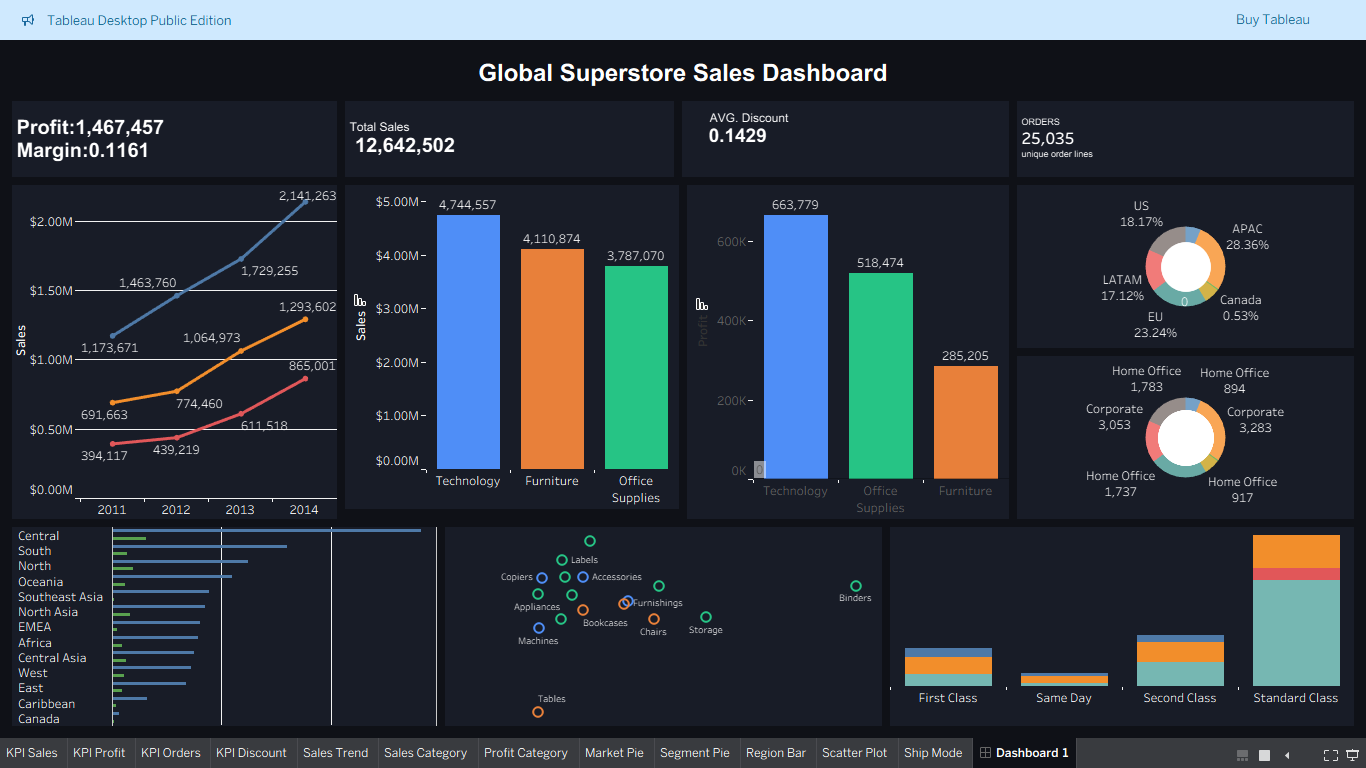
\includegraphics[width=\linewidth]{main_dashboard.png}
\caption{Interactive Tableau dashboard presenting KPIs, trends, and multi-dimensional analysis views.}
\label{fig:dashboard}
\end{figure}

\subsection{Temporal and Segment-Based Trends}

The trend for sales over the last five years (2012-2015) indicates that sales have been steadily rising, suggesting a positive growth trajectory for the business. However, the growth rate varies from customer to customer. The Consumer segment makes the bigger sales volume during the period covered by the study followed by the Corporate and Home Office segments.

Although sales have improved over time, profit growth doesn't necessarily go hand-in-hand, which means that more revenue does not result in better profit. This finding is consistent with previous research which indicated that higher sales volumes with aggressive discounting approach are not necessarily proportionately related to gains on the financial side of the business. \cite{andel2014discounting}.

\subsection{Category Profitability and Performance Disparities}

A comparative analysis of product categories reveals significant disparities in profitability. As shown in Fig.~\ref{fig:category_profit}, the Technology and Office Supplies categories generate consistently positive profits, reflecting efficient pricing and cost management strategies.

The Furniture category is a critical anomaly, however, in contrast. It is a substantial part of the total sales, but, in some cases, it has negative profitability. Some of the sub-categories, in the Furniture line, are in loss, possibly because of high discount or higher operating costs.
\begin{figure}[htbp]
\centering
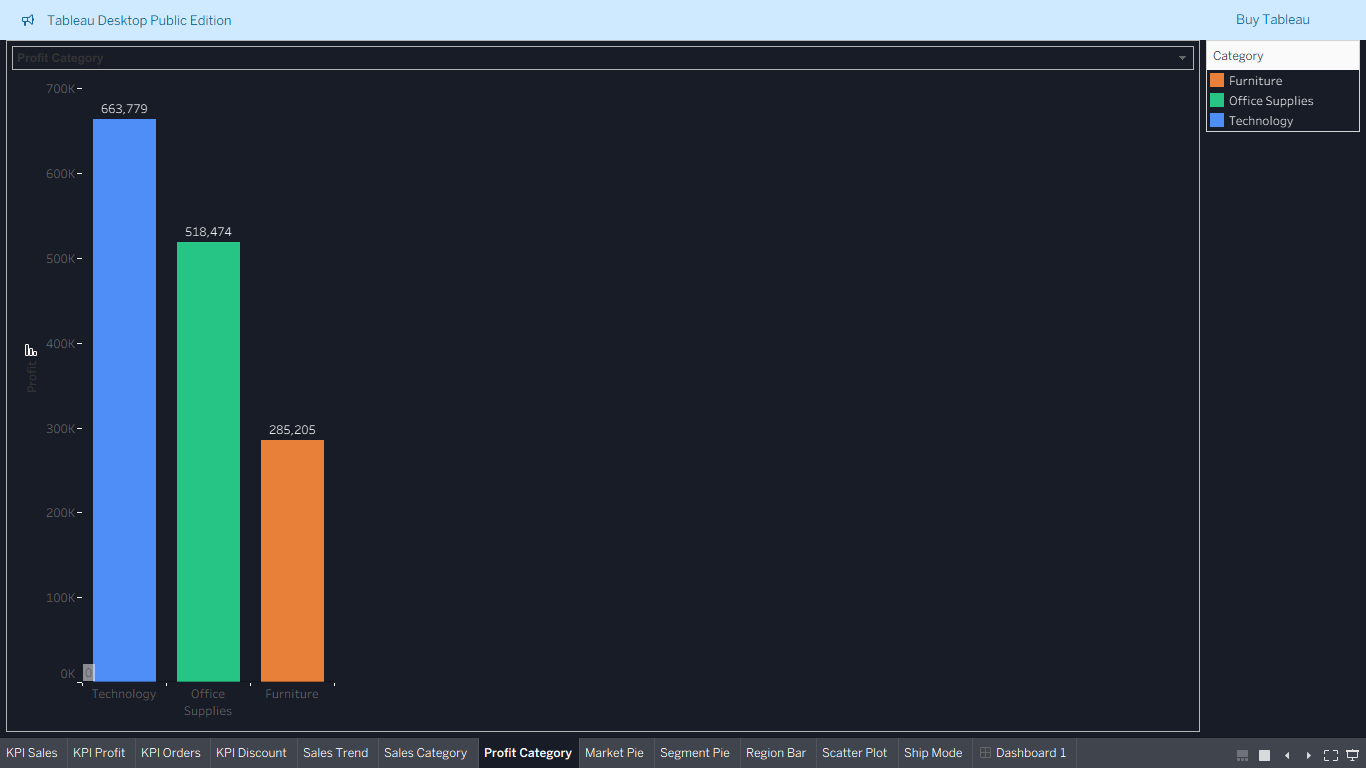
\includegraphics[width=\linewidth]{category_profit.png}
\caption{Profit distribution across product categories, highlighting negative profitability in Furniture.}
\label{fig:category_profit}
\end{figure}









\subsection{Impact of Discounts on Profitability}

The scatter plot analysis gives a greater understanding of the relationship between the discount rates and profit margins. According to the example in Figure~\ref{fig:scatter_discount} a high negative relation exists between the discount level and profitability. The dots for higher discount rates are generally located in the red area of the profit, which is in line with the theory that over discounting has a negative effect on the profit.

This is especially true for certain sub-categories of Furniture where high discounting can result in huge losses. The fact that there is a linear trend line that also confirms this inverse relationship, further strengthens the theory that discounting can lead to reduced overall profitability.
\cite{andel2014discounting}.

\begin{figure}[htbp]
\centering
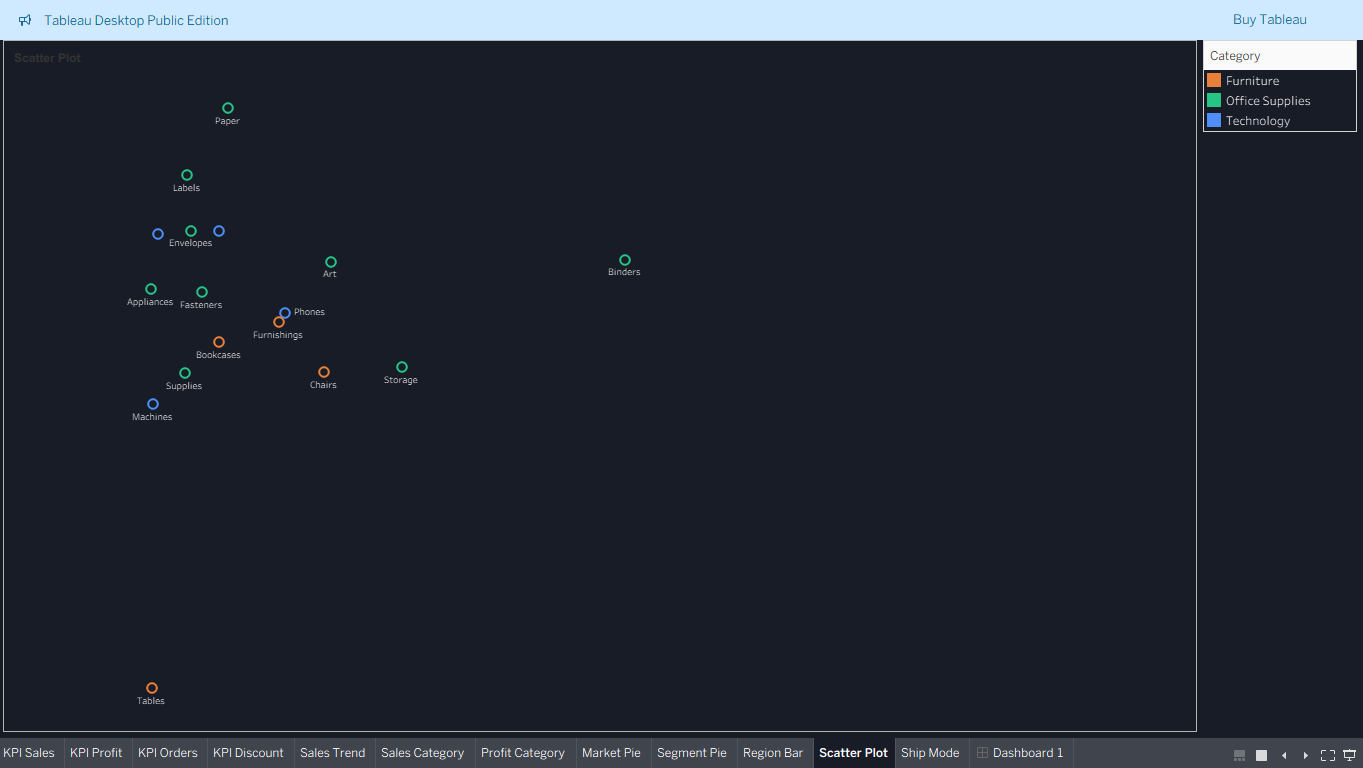
\includegraphics[width=\linewidth]{discount_vs_profit.png}
\caption{Scatter plot showing the negative correlation between discount rates and profit margins.}
\label{fig:scatter_discount}
\end{figure}

\subsection{Role of Interactive Exploration}

One of the major benefits of the dashboard that was implemented is that it allows for interactive exploration of the data via coordinated views. Highlight and filter actions enable the user to dynamically explore relationships between the data across multiple dimensions. For example, if you choose Furniture, the data points for Furniture will be selected, so you can easily see that there are loss-making sub-categories if any, in a flash.

Like this, user will be able to filter specific customer segments and market regions, thus allowing them to isolate trends and analyze the performance of specific market regions. This interactive capability fits with the principles of Visual Analytics and gives a possibility of effective exploration and enhancement of the effectiveness of decision-making.\cite{heer2010interactive}.

\subsection{Discussion}

The findings indicate that although the company has good sales performance, profitability is largely determined by the operational decision-making processes, including discounting policies and management of product categories. The adverse effect of high discounts, especially in the Furniture category is indicative of the necessity of more balanced pricing approaches.

Moreover, the results draw attention and significance of combining various visualization tools as a single dashboard. The analysis using KPIs, trend analysis, categorical comparison, and correlation plot offers a complete analytical framework. Interactivity also contributes to the enhancement of the analytical process as users are able to reveal some hidden patterns and relationships that might not be clearly visible in the case of the static reports.

On balance, the paper confirms that interactive dashboards are an effective decision-support tool that allows organizations to shift towards more exploratory and diagnostic analysis of data.

\section*{Conclusion}
This paper outlined the design and implementation of a interactivity Tableau dashboard used in analyzing sales performance and profitability using the Global Superstore dataset. A holistic analytical framework was created that would assist in efficient business intelligence and decision-making through data preprocessing, formulation of metrics, and multi-dimensional visualization techniques.

The findings reveal that, although the overall sales show a steady upward trend throughout the period under analysis, the profitability is not proportional. This difference is mainly ascribed to operational issues including aggressive discounting policies and category inefficiencies. Specifically, the Furniture category was recognized as a critical area of concern, where the high volume of sales are counterbalanced by negative profit margins. Moreover, the correlation analysis showed the existence of a strong negative relationship between discount rates and profitability, which validated the hypothesis that excessive discounting adversely affects financial performance in a strong negative manner.

The introduction of coordinated visualizations and interactive actions in dashboard allowed to explore the complex relationships in the dataset in an efficient way. Users can easily move between high-level summaries to detailed information, allowing them to quickly identify performance bottlenecks and make decisions using data. This contributes to the efficiency of interactive dashboards as a viable solution to visual analytics in business real-life contexts.

This study has a number of weaknesses despite its contributions. The analysis is done based on one single dataset and does not factor in external factors, which may have affected profitability, such as market competition, supply chain constraints, and customer behavior dynamism. Also, the existing dashboard is geared towards descriptive and diagnostic analytics, without the use of predictive or prescriptive modeling techniques.

Future work can build upon this research by incorporating machine learning models to forecast demand, segment customers and optimize prices. The use of real-time data-streams and enhanced analytical functionality could also contribute to making the dashboard a more useful comprehensive decision-support system.

Finally, the paper will emphasize the significance of preprocessing data, creating visualization designs, and interactivity to reveal meaningful insights in complex datasets. The proposed dashboard illustrates how visual analytics could be successfully utilized to identify the key performance drivers, uncover inefficiencies, and support the strategic decision-making in a data-driven environment.

\bibliographystyle{IEEEtran}
\bibliography{references}

\end{document}




